\documentclass[xcolor={svgnames}]{beamer}

\setbeameroption{hide notes} 

%\usetheme{NLP}
\usetheme{boxes}
\useoutertheme{infolines}
\setbeamertemplate{background}[grid][step=10pt]

\usepackage{graphicx}
\usepackage{lmodern}

\usepackage{soul}

\usepackage{amsmath,amsthm,amssymb}   

\usepackage{listings}

%\usepackage{algorithm,algorithmic}

\usepackage{tikz}
\usetikzlibrary{calc,positioning,shapes,shadows,arrows,tikzmark}

% Text
\newcommand{\todo}[1]{\hl{\textbf{TODO:} #1}}
\newcommand{\citationneeded} {\ensuremath{^{[\textrm{citation needed}]}}}


%Math Operators
%\DeclareMathOperator {\argmax} {argmax}
%\DeclareMathOperator {\argmin} {argmin}
\DeclareMathOperator {\sgn} {sgn}
\DeclareMathOperator {\trace} {tr}
\DeclareMathOperator{\E} {\mathbb{E}}
\DeclareMathOperator{\Var} {Var}
\DeclareMathOperator{\diag} {diag}
\DeclareMathOperator{\triu} {triu}
\DeclareMathOperator{\mult} {Multinomial}
\DeclareMathOperator{\normalt} {Normal}
\DeclareMathOperator{\cvec} {cvec}

\newcommand{\ud}{\, \mathrm{d}}
\newcommand{\diff}[1] {\frac{\partial}{\, \partial #1}}
\newcommand{\difff}[2] {\frac{\partial^2}{\, \partial #1\, \partial #2}}
\newcommand{\diffn}[2] {\frac{\partial^{#2}}{\, \partial {#1}^{#2}}}
\newcommand{\tuple}[1] {\langle #1 \rangle}
\newcommand{\innerprod}[2] {\langle #1, #2 \rangle}

% Constants/etc.
\renewcommand{\Re} {\mathbb{R}}
\newcommand{\Cm} {\mathbb{C}}
\newcommand{\Qm} {\mathbb{Q}}
\newcommand{\half} {\frac{1}{2}}

\newcommand{\inv}[1] {{#1}^{-1}}

\newcommand{\normal}[2] {\mathcal{N}(#1, #2)}
\newcommand{\mL} {\mathcal{L}}

\newcommand\eqdef{\ensuremath{\stackrel{\rm def}{=}}} % Equal by definition
\newcommand\refeqn[1]{(\ref{eqn:#1})}
\newcommand\sD{\ensuremath{\mathcal{D}}}
\newcommand\sM{\ensuremath{\mathcal{M}}}
\newcommand\refapp[1]{Appendix~\ref{sec:#1}}
\newcommand\refthm[1]{Theorem~\ref{thm:#1}}
\newcommand\sigmamin{\sigma_\text{\rm min}}
\newcommand\sigmamax{\sigma_\text{\rm max}}
\newcommand\op{{\text{\rm op}}}
\newcommand\BP{\ensuremath{\mathbb{P}}}
\newcommand\reflem[1]{Lemma~\ref{lem:#1}}

\newcommand{\sidenote}[1]{\begin{itemize} \item #1 \end{itemize}}
\newcommand{\hlmath}[1]{\textrm{\color{blue}\ensuremath{#1}}}

\pgfdeclarelayer{bg}
\pgfsetlayers{bg,main}
\newcommand{\obj}[1]{%
    {%
    \begin{minipage}{6cm}
      #1
    \end{minipage}
    }
}
\newcommand{\objw}[2]{%
    {%
    \begin{minipage}{#1}
      #2
    \end{minipage}
    }
}
\tikzstyle{box}=[scale=0.8,rectangle,fill=white,draw=black]
\tikzstyle{loop}=[smooth,dashed,in=-90,out=-90,looseness=0.75]

\makeatletter
\newcommand*{\centerfloat}{%
  \parindent \z@
  \leftskip \z@ \@plus 1fil \@minus \textwidth
  \rightskip\leftskip
  \parfillskip \z@skip}
\makeatother

% Tensor powers
\newcommand{\tp}[1] {^{\otimes #1}}

% Matrix Perturbation
\newcommand{\pinv}[1] {#1^{\dagger}}
\newcommand{\Ap} {\hat{A}}
\newcommand{\Bp} {\hat{B}}
\newcommand{\Up} {\hat{U}}
\newcommand{\Vp} {\hat{V}}
\newcommand{\Xp} {\hat{X}}
\newcommand{\Wp} {\hat{W}}
\newcommand{\cM} {\mathcal{M}}
\newcommand{\cMp} {\hat{\mathcal{M}}}
\newcommand{\Mp} {\hat{M}}
\newcommand{\Zp} {\hat{Z}}
\newcommand{\vp} {\hat{v}}
\newcommand{\lambdap} {\hat{\lambda}}
\newcommand{\sigmap} {\hat{\sigma}}
\newcommand{\mup} {\hat{\mu}}
\newcommand{\cnd}[1] {\kappa(#1)}
\newcommand{\aerr}[1] {\varepsilon_{#1}}
\newcommand{\rerr}[1] {\delta_{#1}}
\newcommand{\serr}[1] {\alpha_{#1}}
\newcommand{\berr}[1] {\beta_{#1}}
\newcommand{\gap}[1] {\Delta_{#1}}

% Keywords
\newcommand{\Pairs}{\mathrm{Pairs}}
\newcommand{\Triples}{\mathrm{Triples}}



% these will be used later in the title page
\title[Spectral Experts]{Spectral Experts for Estimating Mixtures of Linear Regressions}
\author[Chaganty, Liang]{%
    Arun Tejasvi Chaganty\\
    Percy Liang
}
\institute{Stanford University}

\begin{document}

% "Beamer, do the following at the start of every section"
\AtBeginSection[] 
{%
\begin{frame}<beamer> 
\frametitle{Outline} % make a frame titled "Outline"
\tableofcontents[currentsection]  % show TOC and highlight current section
\end{frame}
}

\begin{frame}
  \titlepage
\end{frame}

\begin{frame}
  \frametitle{Latent Variable Models}


  \splitcolumn{%
    \begin{itemize} 
      \item {\bf Generative Models} \tikzmark{gen}
        \uncover<2->{%
        \begin{itemize}
          \item Gaussian Mixture Models
          \item Hidden Markov Models
          \item Latent Dirichlet Allocation
          \item PCFGs
          \item \dots
        \end{itemize}
        }
      \item<3-> {\bf Discriminative Models} \tikzmark{disc}
        \uncover<4->{%
        \begin{itemize}
          \item Mixture of Experts
          \item Latent CRFs
          \item Discriminative LDA
          \item \dots
          \item {\em Easy to include features and tend to be more accurate.}
        \end{itemize}
        }
      \end{itemize}
  }{%
  \begin{tikzpicture}[remember picture, overlay]
    \draw[use as bounding box] (current page.north west) rectangle (current page.south east);
    \point{mark}{(2cm,0)};
    \point{gen}{(pic cs:gen)};
    \point{disc}{(pic cs:disc)};
    \point{a}{((pic cs:gen) -| mark)};
    \point{b}{((pic cs:disc) -| mark)};
    %\node<1-> at (a) {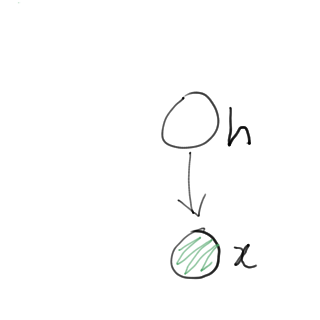
\includegraphics[width=\textwidth,height=3cm,keepaspectratio]{figures/gen.png}};
    %\node<1-> at (b) {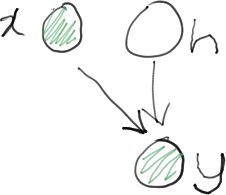
\includegraphics[width=\textwidth,height=3cm,keepaspectratio]{figures/disc.png}};
  \end{tikzpicture}
  }

\end{frame}

\begin{frame}
  \frametitle{Parameter Estimation is Hard}

  \begin{tikzpicture}
    % x, y
    \node[style=box] at (0,-1.5) {\objw{12cm}{%
    \includegraphics<1>[width=\textwidth,height=6cm,keepaspectratio]{figures/likelihood.png}
    \includegraphics<2>[width=\textwidth,height=6cm,keepaspectratio]{figures/likelihood-mle.png}
    \includegraphics<3>[width=\textwidth,height=6cm,keepaspectratio]{figures/likelihood-em.png}
    \includegraphics<4>[width=\textwidth,height=6cm,keepaspectratio]{figures/likelihood-mom.png}
      \hfill{\em expected negative log-likelihood}
      }};
  \end{tikzpicture}

  % Simple message: MLE is consistent but intractable, EM is efficient not but consistent. Can we get something in between.

  \begin{itemize}
    \item<1-> Log-likelihood function is non-convex.
    \item<2-> MLE is consistent but intractable.
    \item<3-> Local methods (EM, gradient descent, etc.) are tractable but inconsistent.
    \item<4-> Can we build {\bf efficient yet consistent estimators} that get better with more data?
  \end{itemize}

\end{frame}

\begin{frame}
  \frametitle{Related Work}
  \begin{itemize}
    \item<+-> Method of Moments [Pearson, 1894]
    \item<+-> Observable operator models
    \begin{itemize}
      \item Subspace identification [Ljung, 1987]
      \item Observable operator models [Jaeger, 2000]
      \item {\em Hidden Markov models [Hsu et al, 2009]}
      \item Low-treewidth graphs [Parikh et al., 2012]
      \item Weighted finite state automata [Balle \& Mohri, 2012]
    \end{itemize}
     \item<+-> Parameter Estimation
  \begin{itemize}
    \item Mixture of Gaussians [Kalai/Moitra/Valiant, 2010]
    \item {\bf Mixture models, HMMs [Anandkumar/Hsu/Kakade, 2012]}
    \item Latent Dirichlet Allocation [Anandkumar/Hsu/Kakade, 2012]
    \item Stochastic block models [Anandkumar/Ge/Hsu/Kakade, 2012]
    \item Linear Bayesian networks [Anandkumar/Hsu/Javanmard/Kakade, 2012]
  \end{itemize}
  \end{itemize}
\end{frame}

\begin{frame}
  \frametitle{Aside: Tensor Operations}
  \begin{tikzpicture}
    % x, y
    \node<1->[style=box] (defn) at (0,0) {\objw{6cm}{%
    \begin{align*}
        \action<1->{%
        x\tp{3}_{ijk} &= x_i x_j x_k \comment{tensoring}\\
        }
        \action<2->{%
        \innerp{A}{B} &= \sum_{ijk} A_{ijk} B_{ijk} \comment{inner product}\\
        }
        \action<3->{%
        A(u)_{ij} &= \sum_{k} A_{ijk} u_k \comment{projection}\\
        }
        \action<4->{%
        A(u,v)_{i} &= \sum_{jk} A_{ijk} u_j v_k \comment{projection} \\
        }
      \end{align*}
    }};
    \tikzcube{black,fill=white}{(6,2,0)}{1}{1}{1};
    %\node (pt) at (5.75,1.75,0) {$\hlmath{\times}$};
    \uncover<3->{%
    \tikzrect{black,fill=white}{(6,0)}{1}{1};
    }
    \uncover<4->{%
    \tikzrect{black,fill=white}{(6,-2)}{0.1}{1};
    }
  \end{tikzpicture}

\end{frame}

\begin{frame}
  \frametitle{Example: Gaussian Mixture Model}
  \begin{tikzpicture}
    % x, y
    \node<1->[style=box] (defn) at (0,0) {\objw{6cm}{%
    \begin{itemize} 
      \item Generative process:
      \begin{align*}
        h &\sim \Mult(\pi) \\
        x &\sim \normal{\beta_h}{\sigma^2}.
      \end{align*}
    \end{itemize}
    }};
    \node<1->[style=box] (models) at (6,0) {\objw{6cm}{%
      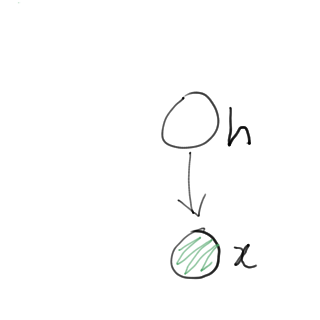
\includegraphics[width=0.45\textwidth,height=3cm,keepaspectratio]{figures/gen.png}
      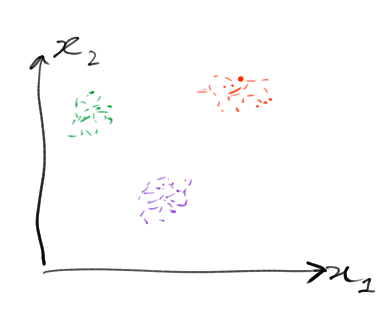
\includegraphics[width=0.45\textwidth,height=3cm,keepaspectratio]{figures/mog.png}
    }};

    \node<2->[style=box,below=0.1cm of defn] {\objw{6cm}{%
    \begin{itemize} 
      \item Moments:
    \begin{align*}
        \action<2->{%
        \E[x|h] &= \beta_h \\
        }
        \action<3->{%
        \E[x] &= \sum_h \pi_h \beta_h \\
        }
        \action<4->{%
        \E[x\tp{2}] &= \sum_h \pi_h (\beta_h \beta_h^T) \\
                    &= \sum_h \pi_h \beta_h{\tp{2}} \\
                    }
        \action<5->{%
        \E[x\tp{3}] &= \sum_h \pi_h \beta_h\tp{3}.
        }
      \end{align*}
    \end{itemize}
    }};
    %\tikzrect{1}{1};
    \uncover<4->{%
    \tikzrect{black,fill=white}{(6,-2)}{1}{1};
    \node at (7,-2.5) {$\E[x\tp{2}]$};
    \node at (4.5,-2.5) {$d$};
    }
    \uncover<5->{%
    \tikzcube{black,fill=white}{(6,-4,0)}{1}{1}{1};
    \node at (7,-4.5,0) {$\E[x\tp{3}]$};
    \node at (4.5,-4.5) {$d$};
    \node at (4.5,-4.5) {$d$};
    }
  \end{tikzpicture}

\end{frame}

\begin{frame}
  \frametitle{Example: Gaussian Mixture Model}
  \begin{tikzpicture}
    % x, y
    \node<1->[style=box] (moments) at (0,0) {\objw{6cm}{%
      If $\beta_h$ are orthogonal;
      \begin{align*}
        \E[x\tp{3}] &= \sum_{h=1}^k \pi_h \beta_h\tp{3}. 
      \end{align*}
    }};
    \node<1->[style=box] (models) at (6,0) {\objw{6cm}{%
      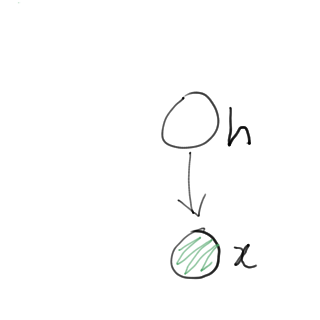
\includegraphics[width=0.45\textwidth,height=3cm,keepaspectratio]{figures/gen.png}
      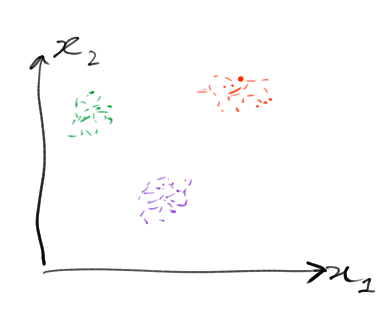
\includegraphics[width=0.45\textwidth,height=3cm,keepaspectratio]{figures/mog.png}
    }};

    \node<1-> at (6,-3) {\objw{6cm}{%
    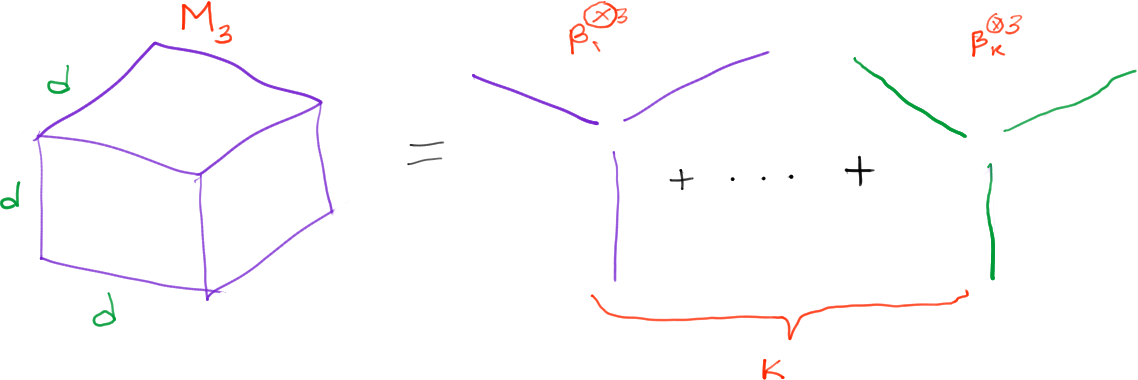
\includegraphics[width=\textwidth,height=6cm,keepaspectratio]{figures/tensor.png}
      }};
    \node<2->[style=box] at (0,-3) {\objw{6cm}{%
      $\beta_h$ are eigenvectors!
        \begin{align*}
          \E[x\tp{3}](\beta_h,\beta_h) 
            %&= \sum_{h'=1}^k \pi_{h'} (\beta_{h}^T \beta_{h'})^2 \beta_{h'} \\
            %&= \sum_{h'=1}^k \pi_{h'} \delta_{hh'} \beta_{h'} \\
            &= \pi_{h} \beta_{h}.
        \end{align*}

        \hfill{\em Anandkumar, Hsu, et.\ al (2012)}
      }};
%
%    \node<2>[style=box,below=0.1cm of tensorf] {\objw{12cm}{%
%    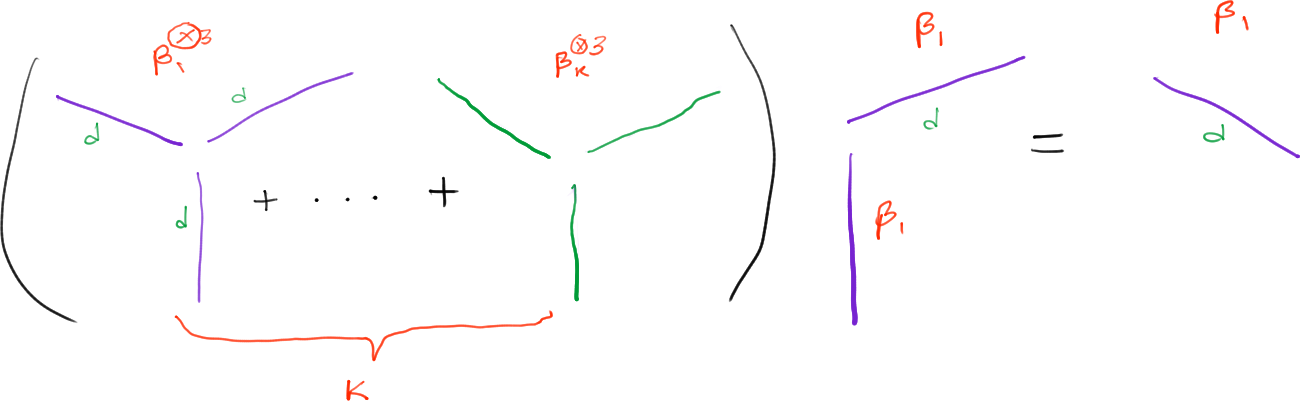
\includegraphics[width=\textwidth,height=6cm,keepaspectratio]{figures/tensor-decomp.png}
%      \hfill {Tensor Power Method}
%      }};
  \end{tikzpicture}
\end{frame}

\begin{frame}
  \frametitle{Generative vs. Discriminative Latent Variable Models}

  \begin{tikzpicture}
    % Tasks.
    \node[style=box] (gen) at (0,0) {\objw{6cm}{%
      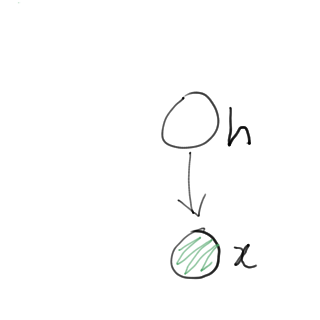
\includegraphics[width=\textwidth,height=3cm,keepaspectratio]{figures/gen.png}\\
      \hfill Generative Models
      }};
    \node[scale=0.7] at (0.5,0.5) {Latent variable};

    \node[style=box] (disc) at (6,0) {\objw{6cm}{%
      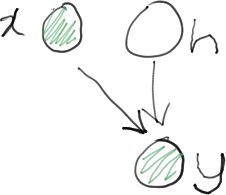
\includegraphics[width=\textwidth,height=3cm,keepaspectratio]{figures/disc.png}\\
      \hfill Discriminative Models
      }};
  \end{tikzpicture}

\end{frame}


\begin{frame}
  \frametitle{Mixture of Linear Regressions}

  \begin{tikzpicture}
    % x, y
    \node[style=box] at (0,0) {\objw{4cm}{%
    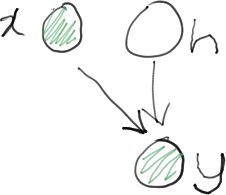
\includegraphics[width=\textwidth,height=4cm,keepaspectratio]{figures/disc.png}
      \begin{itemize}
        \item<2-> $h \sim \Mult(\pi)$.
        \item<4-> $y = \beta_h^T x + \epsilon$.
      \end{itemize}
      }};

    \node[style=box] at (6,0) {\obj{%
    \includegraphics<1>[width=\textwidth,height=6cm,keepaspectratio]{figures/mlr-data-2.png}
    \includegraphics<2>[width=\textwidth,height=6cm,keepaspectratio]{figures/mlr-data-3a.png}
    \includegraphics<3>[width=\textwidth,height=6cm,keepaspectratio]{figures/mlr-data-3b.png}
    \includegraphics<4>[width=\textwidth,height=6cm,keepaspectratio]{figures/mlr-data-4a.png}
    \includegraphics<5>[width=\textwidth,height=6cm,keepaspectratio]{figures/mlr-data-4b.png}
    %\includegraphics<6>[width=\textwidth,height=6cm,keepaspectratio]{figures/mlr-data-4c.png}
    \includegraphics<6>[width=\textwidth,height=6cm,keepaspectratio]{figures/mlr-data-5.png}
      }};
  \end{tikzpicture}
\end{frame}

\begin{frame}
  \frametitle{Mixture of Linear Regressions}

  \begin{tikzpicture}
    \node[style=box] (data) at (0,0) {\obj{%
    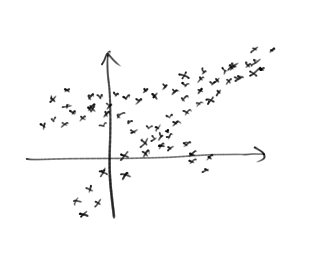
\includegraphics[width=\textwidth,height=6cm,keepaspectratio]{figures/mlr-data-6.png}
      \\{\em Data}
      }};

    % x, y
    \node[style=box] (params) at (7,0) {\objw{4cm}{%
    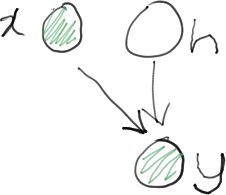
\includegraphics[width=\textwidth,height=4cm,keepaspectratio]{figures/disc.png}
    \\
    {\bf Parameters: $\pi, B$}
    }};

    \draw[->,dashed] (data) -- node[above]{?} (params);


  \end{tikzpicture}
\end{frame}

% \begin{frame}
%   \frametitle{Method of Moments for Generative LVMs.}
% 
%   \begin{tikzpicture}
%     % x, y
%     \node<1->[style=box]  (moments) at (0,0) {\objw{12cm}{%
%       \begin{align*}
%         \underbrace{\E[x]}_{M_1} &= \sum_{h=1}^k \pi_h \beta_h & 
%         \underbrace{\E[x\tp{2}]}_{M_2} &= \sum_{h=1}^k \pi_h \beta_h\tp{2} & 
%         \underbrace{\E[x\tp{3}]}_{M_3} &= \sum_{h=1}^k \pi_h \beta_h\tp{3}. 
%       \end{align*}
%     }};
%     \node<1>[style=box,below=0.1cm of moments] {\objw{12cm}{%
%     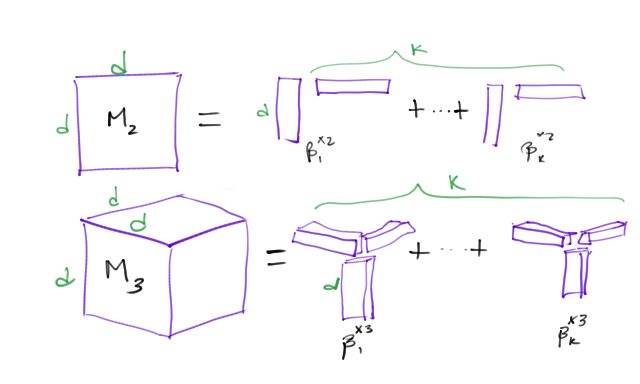
\includegraphics[width=\textwidth,height=6cm,keepaspectratio]{figures/moments.png}
%       }};
%     \node<2->[style=box,below=0.1cm of moments] {\objw{12cm}{%
%       \begin{itemize}
%         \item<2-> {\bf Tensor Power Method} for orthonormal $\beta_h$,
%           \begin{align*}
%             M_3(\beta_h,\beta_h) 
%               &= \sum_{h'=1}^k \pi_{h'} (\beta_{h}^T \beta_{h'})^2 \beta_{h'} \\
%               &= \sum_{h'=1}^k \pi_{h'} \delta_{hh'} \beta_{h'} \\
%               &= \pi_{h'} \beta_{h}.
%           \end{align*}
%         \item<3-> Use $M_2$ to whiten $M_3$.
%       \end{itemize}
%       }};
%   \end{tikzpicture}
% 
% \end{frame}

\begin{frame}
  \frametitle{Method of Moments for the Mixture of Linear Regressions.}

  \begin{tikzpicture}
    % x, y
    \node[style=box] at (0,0) {\objw{12cm}{%
        \begin{align*}
          \action<+->{
          y &= \underbrace{\beta_h^T}_{\textrm{random}} x + \epsilon \\
          }
          \action<+->{
            &= \underbrace{\E[\beta_h]^T x}_{\textrm{linear measurement}} + \underbrace{(\beta_h - \E[\beta_h])^T x + \epsilon}_{\textrm{noise}} \\
          }
        \end{align*}
      }};
  \end{tikzpicture}

\end{frame}

\begin{frame}
  \frametitle{Method of Moments for the Mixture of Linear Regressions.}

  \begin{tikzpicture}
    % x, y
    \node[style=box] (measurements) at (0,0) {\objw{12cm}{%
        \begin{align*}
          \action<+->{%
          y &= \underbrace{\innerp{\E[\beta_h]^T}{x}}_{\textrm{linear measurement}} &\quad & + \underbrace{(\beta_h - \E[\beta_h])^T x + \epsilon}_{\textrm{noise}} \\
          }
          \action<+->{%
            y^2 
            &= \innerp{\E[\beta_h\tp{2}]}{x\tp{2}} &+ \textrm{bias} &+ \textrm{noise} \\
          }
          \action<+->{%
          y^3 &= \innerp{\E[\beta_h\tp{3}]}{x\tp{3}} &+ \textrm{bias} &+ \textrm{noise} \\
          }
        \end{align*}

        \uncover<4->{%
        We can use regression to recover $\E[\beta_h\tp{p}]$ from linear measurements.\\
          }
      }};

    \node<5->[style=box,below=0.1cm of measurements.south] (tensor) {\objw{12cm}{%
      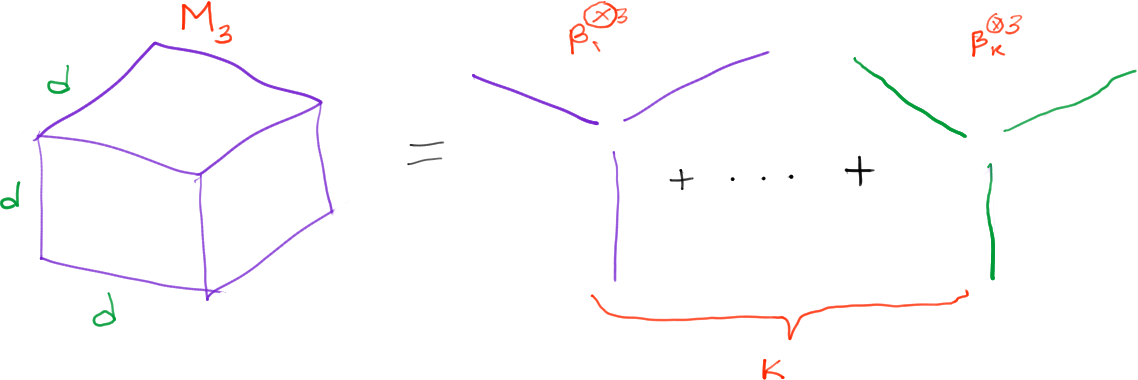
\includegraphics[width=\textwidth,height=3cm,keepaspectratio]{figures/tensor.png}
      }};

  \end{tikzpicture}
\end{frame}

\begin{frame}
  \frametitle{Overview: Spectral Experts}

  \begin{tikzpicture}
    % x, y
    % Nodes
    \node[style=txt] (data1) at (0,0) {$\left\{ x, y \right\}_{(x,y) \in \sD}$};
    \node[style=txt,below=1cm of data1.center] (data2) {$\left\{ x\tp{2}, y^2 \right\}_{(x,y) \in \sD}$};
    \node[style=txt,below=1cm of data2.center] (data3) {$\left\{ x\tp{3}, y^3 \right\}_{(x,y) \in \sD}$};

    \node[style=txt] (m1) at (4,0) {$\E_h\left[\beta_h\right]$};
    \node[style=txt,below=1cm of m1.center] (m2) {$\E_h\left[\beta_h\tp{2}\right]$};
    \node[style=txt,below=1cm of m2.center] (m3) {$\E_h\left[\beta_h\tp{3}\right]$};

    \node[below=0.5cm of m2.center] (params-pos) {};
    \node[style=txt,right=3.0cm of params-pos] (params) {$\pi, B$};

    % Arrows
    \draw[-latex] (data1) -- (m1);
    \draw[-latex] (data2) -- (m2);
    \draw[-latex] (data3) -- (m3);

    % Bias influence
    \draw[-latex,dashed,gray] (m1.east) -- ++(0.1cm,0) -- ++(0,-0.50cm) -- ++(-3.00cm,0) node (bias-1) {} -- ( bias-1 |- m3) -- (m3.west);

    % Mean
    \draw[-latex] (m2.east) -- ++(0.1cm,0) node (tf-1) {} -- (tf-1 |- params-pos) -- node[above,scale=0.5] {tensor factorization} (params);
    \draw[-latex] (m3.east) -- ++(0.1cm,0) node (tf-2) {} -- (tf-2 |- params-pos) -- (params);

    % Box for regression
    \begin{pgfonlayer}{bg}
    \draw[fill=blue,opacity=0.1,dashed] ($(data1.north east) + (-0.1cm,0.1cm)$) rectangle ($(m3.south west) + (0.1cm,-0.1cm)$);
    \end{pgfonlayer}
    \node[style=txt] (reg-label) at ($(data3) !.5! (m3) + (0, -1.0cm)$) {regression};

    % tensor factorization
    \begin{pgfonlayer}{bg}
    \draw[fill=green,opacity=0.1,dashed] ($(m2.north east) + (-0.1cm,0.1cm)$) rectangle ($(params.south west) + (0.1cm,-1.0cm)$);
    \end{pgfonlayer}
    \node (params-mid) at ($(params-pos) !.5! (params)$) {};
    \node[style=txt] at (params-mid |- reg-label) {tensor factorization};
  \end{tikzpicture}
\end{frame}


\begin{frame}
  \frametitle{Method of Moments for the Mixture of Linear Regressions.}

  \begin{tikzpicture}
    % x, y
    \node[style=box] (reg) at (0,0) {\objw{12cm}{%
      \begin{align*}
        \hat\E[\beta_h\tp{2}] &= \arg\min_{M} \left(y^2 - \innerp{M}{x\tp{2}}\right)^2_{(x,y)\in\mathcal{D}} \action<3->{+ \hlmath{\|M\|_{*}}} \\
        \action<3->{%
        \|M\|_{*} &= \sum_i \sigma_i(M).
        }
      \end{align*}
      }};
    \node<2->[style=box,below=0.1 of reg] (measurements) {\objw{12cm}{%
      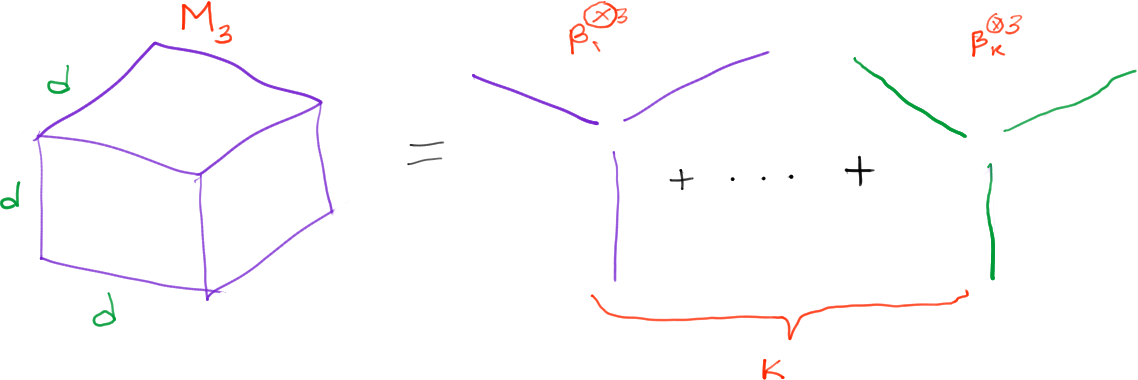
\includegraphics[width=\textwidth,height=6cm,keepaspectratio]{figures/tensor.png}
      }};
  \end{tikzpicture}
\end{frame}

\begin{frame}
  \frametitle{Overview: Spectral Experts}

  \begin{tikzpicture}
    % x, y
    % Nodes
    \node[style=txt] (data1) at (0,0) {$\left\{ x, y \right\}_{(x,y) \in \sD}$};
    \node[style=txt,below=1cm of data1.center] (data2) {$\left\{ x\tp{2}, y^2 \right\}_{(x,y) \in \sD}$};
    \node[style=txt,below=1cm of data2.center] (data3) {$\left\{ x\tp{3}, y^3 \right\}_{(x,y) \in \sD}$};

    \node[style=txt] (m1) at (4,0) {$\E_h\left[\beta_h\right]$};
    \node[style=txt,below=1cm of m1.center] (m2) {$\E_h\left[\beta_h\tp{2}\right]$};
    \node[style=txt,below=1cm of m2.center] (m3) {$\E_h\left[\beta_h\tp{3}\right]$};

    \node[below=0.5cm of m2.center] (params-pos) {};
    \node[style=txt,right=3.0cm of params-pos] (params) {$\pi, B$};

    % Arrows
    \draw[-latex] (data1) -- (m1);
    \draw[-latex] (data2) -- node[above,scale=0.5] {low rank} (m2);
    \draw[-latex] (data3) -- node[above,scale=0.5] {low rank} (m3);

    % Bias influence
    \draw[-latex,dashed,gray] (m1.east) -- ++(0.1cm,0) -- ++(0,-0.50cm) -- ++(-3.00cm,0) node (bias-1) {} -- ( bias-1 |- m3) -- (m3.west);

    % Mean
    \draw[-latex] (m2.east) -- ++(0.1cm,0) node (tf-1) {} -- (tf-1 |- params-pos) -- node[above,scale=0.5] {tensor factorization} (params);
    \draw[-latex] (m3.east) -- ++(0.1cm,0) node (tf-2) {} -- (tf-2 |- params-pos) -- (params);

    % Box for regression
    \begin{pgfonlayer}{bg}
    \draw[fill=blue,opacity=0.1,dashed] ($(data1.north east) + (-0.1cm,0.1cm)$) rectangle ($(m3.south west) + (0.1cm,-0.1cm)$);
    \end{pgfonlayer}
    \node[style=txt] (reg-label) at ($(data3) !.5! (m3) + (0, -1.0cm)$) {regression};

    % tensor factorization
    \begin{pgfonlayer}{bg}
    \draw[fill=green,opacity=0.1,dashed] ($(m2.north east) + (-0.1cm,0.1cm)$) rectangle ($(params.south west) + (0.1cm,-1.0cm)$);
    \end{pgfonlayer}
    \node (params-mid) at ($(params-pos) !.5! (params)$) {};
    \node[style=txt] at (params-mid |- reg-label) {tensor factorization};
  \end{tikzpicture}
\end{frame}

\begin{frame}
  \frametitle{Sample Complexity}

  \begin{tikzpicture}
    % x, y
    % Nodes
    \node[style=txt] (data1) at (0,0) {$\left\{ x, y \right\}_{(x,y) \in \sD}$};
    \node[style=txt,below=1cm of data1.center] (data2) {$\left\{ x\tp{2}, y^2 \right\}_{(x,y) \in \sD}$};
    \node[style=txt,below=1cm of data2.center] (data3) {$\left\{ x\tp{3}, y^3 \right\}_{(x,y) \in \sD}$};

    \node[style=txt] (m1) at (4,0) {$\E_h\left[\beta_h\right]$};
    \node[style=txt,below=1cm of m1.center] (m2) {$\E_h\left[\beta_h\tp{2}\right]$};
    \node[style=txt,below=1cm of m2.center] (m3) {$\E_h\left[\beta_h\tp{3}\right]$};

    \node[below=0.5cm of m2.center] (params-pos) {};
    \node[style=txt,right=3.0cm of params-pos] (params) {$\pi, B$};

    % Arrows
    \draw[-latex] (data1) -- (m1);
    \draw[-latex] (data2) -- node[above,scale=0.5] {low rank} (m2);
    \draw[-latex] (data3) -- node[above,scale=0.5] {low rank} (m3);

    % Bias influence
    \draw[-latex,dashed,gray] (m1.east) -- ++(0.1cm,0) -- ++(0,-0.50cm) -- ++(-3.00cm,0) node (bias-1) {} -- ( bias-1 |- m3) -- (m3.west);

    % Mean
    \draw[-latex] (m2.east) -- ++(0.1cm,0) node (tf-1) {} -- (tf-1 |- params-pos) -- node[above,scale=0.5] {tensor factorization} (params);
    \draw[-latex] (m3.east) -- ++(0.1cm,0) node (tf-2) {} -- (tf-2 |- params-pos) -- (params);

    % Box for regression
    \begin{pgfonlayer}{bg}
    \draw[fill=blue,opacity=0.1,dashed] ($(data1.north east) + (-0.1cm,0.1cm)$) rectangle ($(m3.south west) + (0.1cm,-0.1cm)$);
    \end{pgfonlayer}
    \node[style=txt] (reg-label) at ($(data3) !.5! (m3) + (0, -1.0cm)$) {regression};

    % tensor factorization
    \begin{pgfonlayer}{bg}
    \draw[fill=green,opacity=0.1,dashed] ($(m2.north east) + (-0.1cm,0.1cm)$) rectangle ($(params.south west) + (0.1cm,-1.0cm)$);
    \end{pgfonlayer}
    \node (params-mid) at ($(params-pos) !.5! (params)$) {};
    \node[style=txt] (tf-label) at (params-mid |- reg-label) {tensor factorization};

    % Error bounds
    \node<2->[style=txt,below=0.1em of reg-label] {$O\left( k \|x\|^{12} \|\beta\|^{6} \|\E[\epsilon^2]\|^{6} \right)$};
    \node<3->[style=txt,below=0.1em of tf-label] {$O\left( \frac{k \pi_{\max}^2}{\sigma_k(M_2)^5} \right)$};

  \end{tikzpicture}
\end{frame}

\begin{frame}
  \frametitle{Experimental Insights}

  \begin{tikzpicture}
    % x, y
    \node (em) at (-3,-0.5) {%
      \includegraphics<1>[width=\textwidth,height=5cm,keepaspectratio]{figures/1-8-3.png}
      \includegraphics<2>[width=\textwidth,height=5cm,keepaspectratio]{figures/1-8-3-em.png}
      \includegraphics<3>[width=\textwidth,height=5cm,keepaspectratio]{figures/1-8-3-spec.png}
      \includegraphics<4->[width=\textwidth,height=5cm,keepaspectratio]{figures/1-8-3-specm.png}
      };
    % x, y
    \node<2-> at (3,-0.5) {%
      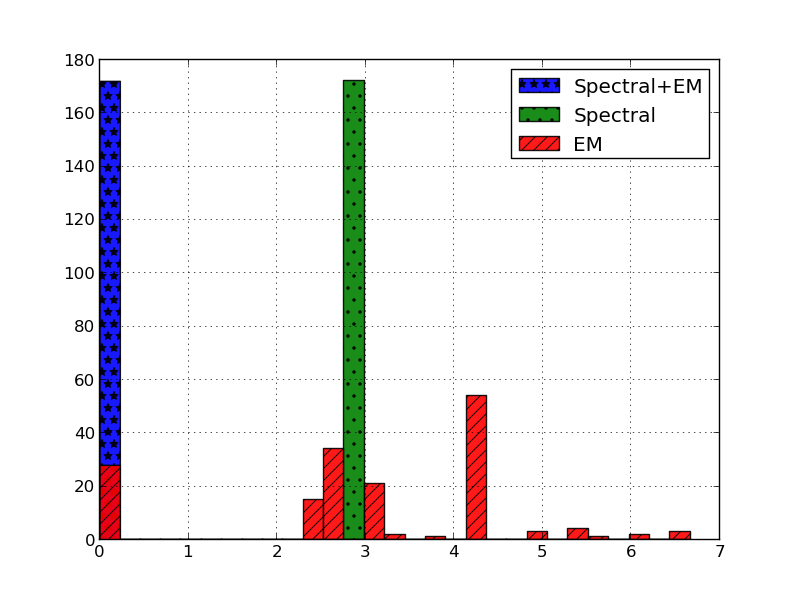
\includegraphics[width=\textwidth,height=5cm,keepaspectratio]{figures/hist.png}
    };

    \node[above=0.1 cm of em] {\objw{3cm}{%
      \begin{align*}
        y &= \beta^T 
            \begin{bmatrix} 
              1 \\
              t \\
              t^4 \\
              t^7
            \end{bmatrix} + \epsilon
      \end{align*}
      }};
  \end{tikzpicture}
\end{frame}

\begin{frame}
  \frametitle{Experimental Insights}

\begin{small}
  \begin{tabular}{r r r c c c}
\hline
%$b$ & 
$d$ & $k$ & Spectral & EM & Spectral + EM \\
\hline
  %1 & 
  4 & 2 & 2.45 $\pm$ 3.68 & 0.28 $\pm$ 0.82 & {\bf 0.17 $\pm$ 0.57} \\
  %2 & 
  5 & 2 & 1.38 $\pm$ 0.84 & {\bf 0.00 $\pm$ 0.00} & {\bf 0.00 $\pm$ 0.00} \\
  %2 & 
  5 & 3 & 2.92 $\pm$ 1.71 & 0.43 $\pm$ 1.07 & {\bf 0.31 $\pm$ 1.02} \\
  %2 & 
  6 & 2 & 2.33 $\pm$ 0.67 & 0.63 $\pm$ 1.29 & {\bf 0.01 $\pm$ 0.01} \\
\hline
\end{tabular}
      \end{small}

\end{frame}

\begin{frame}
  \frametitle{Experimental Insights}

  \begin{tikzpicture}
    \node[style=box] at (0,-1.5) {\objw{12cm}{%
      \includegraphics<1>[width=\textwidth,height=6cm,keepaspectratio]{figures/likelihood-mom.png}
      \includegraphics<2>[width=\textwidth,height=6cm,keepaspectratio]{figures/likelihood-mom-em1.png}
      \includegraphics<3>[width=\textwidth,height=6cm,keepaspectratio]{figures/likelihood-mom-em2.png}
        \hfill{\em expected negative log-likelihood}
      }};
  \end{tikzpicture}

\end{frame}


\begin{frame}
  \frametitle{Conclusions}
  \begin{itemize}
    \item {\bf Consistent estimator} for the mixture of linear regressions with {\bf polynomial sample and computational complexity}.
    \item<2-> Derive conditional moments using regression.
    \item<3-> Method of moment estimates can be a good initialization for EM.
  \end{itemize}
\end{frame}

\begin{frame}
  \frametitle{}
    Thank you.
\end{frame}

\end{document}

% TikZ
%\begin{tikzpicture}
%  \node (img1) at (0,0) {\includegraphics[height=0.6\textheight,width=0.4\linewidth,keepaspectratio]{}};
%\end{tikzpicture}

% Notes 
% \note[item]{}

% 2-column
% \begin{columns}
%   \begin{column}{0.48\textwidth}
%     \begin{itemize}
%         \item
%     \end{itemize}
%   \end{column}
%   \hfill
%   \begin{column}{0.48\textwidth}
%     \begin{itemize}
%         \item
%     \end{itemize}
%   \end{column}
% \end{columns}

% TikZ
%\begin{tikzpicture}
%  \node (img1) at (0,0) {\includegraphics[height=0.6\textheight,width=0.4\linewidth,keepaspectratio]{}};
%\end{tikzpicture}

% Notes 
% \note[item]{}

% 2-column
% \begin{columns}
%   \begin{column}{0.48\textwidth}
%     \begin{itemize}
%         \item
%     \end{itemize}
%   \end{column}
%   \hfill
%   \begin{column}{0.48\textwidth}
%     \begin{itemize}
%         \item
%     \end{itemize}
%   \end{column}
% \end{columns}

